\documentclass[fleqn]{article}
\oddsidemargin 0.0in
\textwidth 6.0in
\thispagestyle{empty}
\usepackage{import}
\usepackage{amsmath}
\usepackage{graphicx}
\usepackage{flexisym}
\usepackage{calligra}
\usepackage{amssymb}
\usepackage{bigints} 
\usepackage[english]{babel}
\usepackage[utf8x]{inputenc}
\usepackage{float}
\usepackage[colorinlistoftodos]{todonotes}


\DeclareMathAlphabet{\mathcalligra}{T1}{calligra}{m}{n}
\DeclareFontShape{T1}{calligra}{m}{n}{<->s*[2.2]callig15}{}
\newcommand{\scriptr}{\mathcalligra{r}\,}
\newcommand{\boldscriptr}{\pmb{\mathcalligra{r}}\,}

\definecolor{hwColor}{HTML}{AD53BA}

\begin{document}

  \begin{titlepage}

    \newcommand{\HRule}{\rule{\linewidth}{0.5mm}}

    \center

    \begin{center}
      
\includegraphics[height=11cm, width=11cm]{asu.png}
    \end{center}

    \vline

    \textsc{\LARGE Classical Parts/Field/Matter III}\\[1.5cm]

    \HRule \\[0.5cm]
    { \huge \bfseries Exam 3}\\[0.4cm] 
    \HRule \\[1.0cm]

    \textbf{Behnam Amiri}

    \bigbreak

    \textbf{Prof: Samuel Teitelbaum}

    \bigbreak

    \textbf{{\large \today}\\[2cm]}

    \vfill

  \end{titlepage}

  \begin{itemize}
    \item This exam is available all weekend, but should take you 4-6 hours to complete.
    \item Your solutions must be uploaded to Canvas just as you do with homework.
    \item The exam should be taken without the use of internet (aside from Canvas materials, and email
    in the event that you have questions during the exam).
    \item The only allowed materials are: Griffiths textbook, your math methods textbook, any materials
    on Canvas, and your own hand-written or hand-typed notes.
    \item Do not discuss the midterm problems with anyone until after May $6th, ~ 2022$.
    \item If you get stuck on math, explain the physics as well as you can.  Much of the credit is given 
    for showing how you proceed through the problem and what assumptions you are making.
  \end{itemize}

  \pagebreak

  \begin{enumerate}
    \item \textbf{Problem 1 [25 points]}
    For the questions below, assume our standard reference frames in which the primed frame $\bar{S}$
    moves at velocity $v \hat{x}$ with respect to the unprimed frame $S$. The origins of the coordinate 
    systems overlap at time $t=\bar{t}=0$.
    \begin{enumerate}
      \item A photon has velocity $\bar{u}=(0,0,c)$ relative to the $\bar{S}$ frame. Find the velocity $u$
      of the photon relative to the $S$ frame.

      \item Determine the speed of the photon in the $S$ frame; confirm that it is still equal to $c$.

      \item Suppose the photon has frequency $\bar{\omega}$ in the $\bar{S}$ frame. Write down the momentum
      4-vector $\bar{p}^{\mu}$ for the photon in the $\bar{S}$ frame. Use Lorentz transformations to find the 
      photon energy $E$ and 3-momentum in the $S$ frame.
    \end{enumerate}


    \begin{center}
      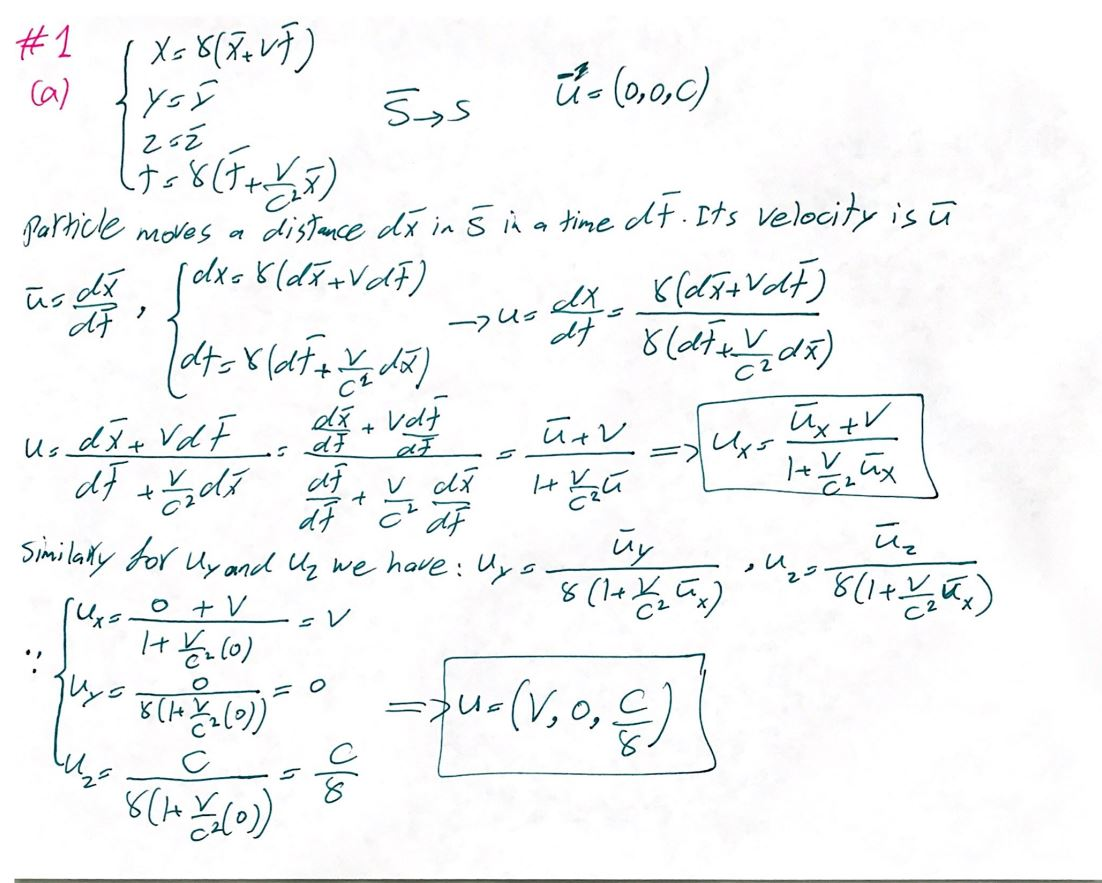
\includegraphics[height=16cm, width=17cm]{1A.JPG}
    \end{center}

    \pagebreak

    \begin{center}
      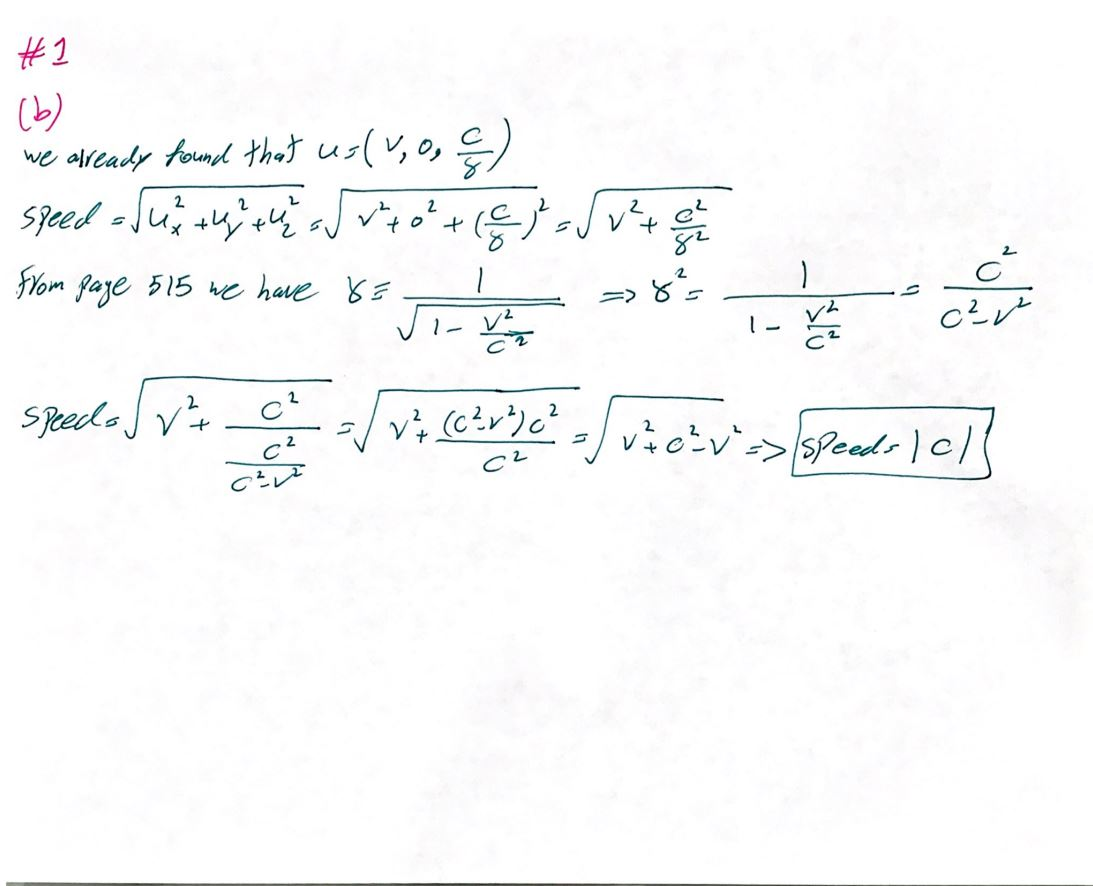
\includegraphics[height=16cm, width=17cm]{1B.JPG}
    \end{center}
    
    \pagebreak

    \begin{center} 
      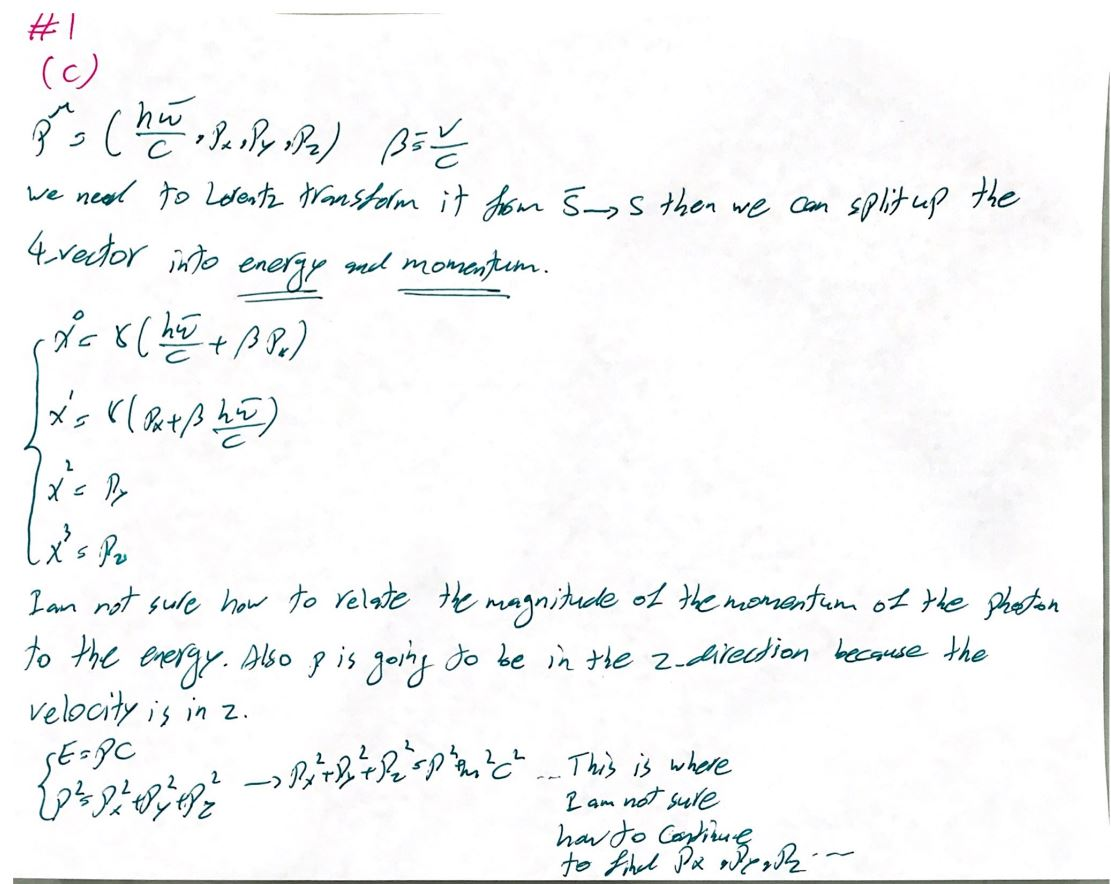
\includegraphics[height=16cm, width=17cm]{1C.JPG}
    \end{center}

    \textbf{Please note that I meant to use $\hbar$ instead of $h$.}

    \pagebreak

    \item \textbf{Problem 2 [25 points]}
    At our CXFEL tour I went over how Inverse Compton scattering can be used to produce x-rays, as
    in the Compact X-ray Light Source in the Biodesign $C$ building. In this problem you will reproduce
    some of the results I derived in lecture. In a simplified picture, suppose that a photon and an electron
    have a direct collision with each other, and the scattered photon propagates opposite to the initial
    direction. The electrons energy is reduced, while the photon’s energy is increased. With knowledge
    of the initial electron energy $E_{e,i}$ and the initial frequency of the photon $\omega_{p, i}$, we aim 
    to find the final frequency of the photon $\omega_{p,f}$ after the collision. I will walk you through the 
    calculation, and you fill in the details.
    \begin{enumerate}
      \item Suppose the initial photon 3-momentum is $p_{p,i}=\hbar k=\hbar \dfrac{\omega}{c} \hat{x}$
      and the initial (relativistic) electron 3-momentum is $p_{e,i}=-p_{e,i} \hat{x}$. Write down the 
      corresponding momentum 4-vectors $p^{\mu}_{p,i}$ and $p^{\mu}_{e,i}$. Recall that the energy of a 
      photon is $E=\hbar \omega$.

      \item We will transform into the primed frame in which the electron is at rest, in which case the
      electron’s momentum 4-vector is understood to be $\bar{p}_{e,i}=\bigg( \bar{E}_{e,i}/c, 0,0,0 \bigg)$.
      Write down the Lorenz-transformed photon momentum 4-vector $\bar{p}_{p,i}$ in this frame. There is 
      nothing to “solve” here; just write it down in terms of the usual $\gamma =\gamma_v$. Be mindful of 
      signs; they are important.

      \item Although there is in principle a Compton frequency shift, we will assume that it is small enough
      to be ignored $(\hbar \bar{\omega}_{p,i} << m_0 c^2)$. Under that assumption, the new momentum in the rest frame
      simply reverses direction. Write down the new momentum 4-vector after the collision, $\bar{p}^{\mu}_{p,f}$.


      \item Now do the Lorentz transformation back into the unprimed lab frame and solve for the final
      momentum 4-vector of the photon, $p^{\mu}_{p,f}$.

      \item Finally, show that the new frequency of the photon is approximately $\omega_{p,f} \approx 4 \gamma^2 \omega_{p,i}$.
      (Note that $\gamma \approx E_{e,i}/m_0 c^2$).

    \end{enumerate}
    Now you know how ASU Compact X-ray Light Source works!

    \begin{center}
      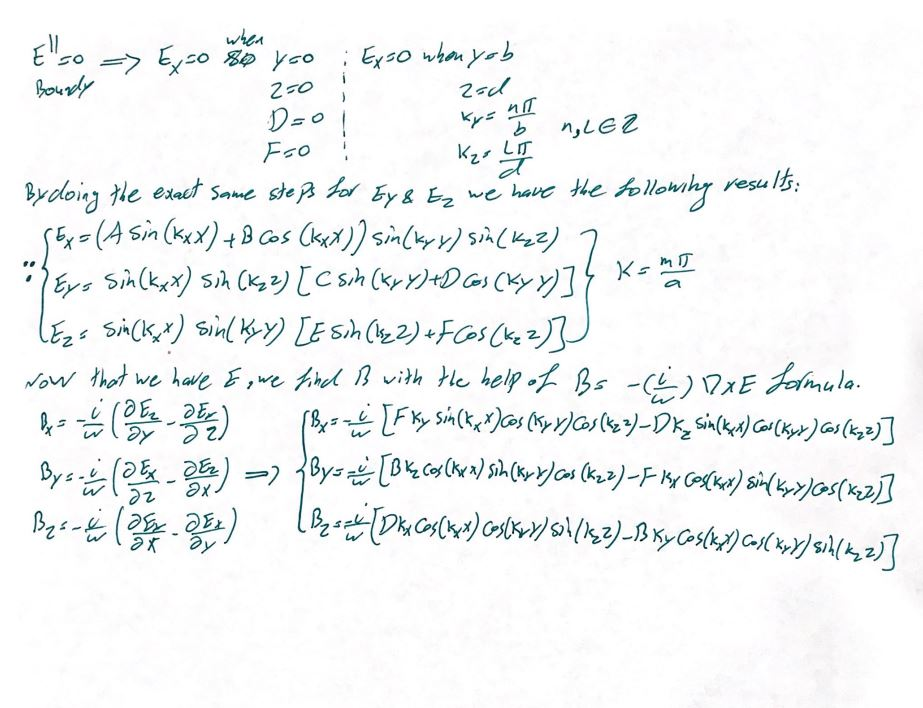
\includegraphics[height=16cm, width=17cm]{2.JPG}
    \end{center}

    \pagebreak


    \item \textbf{Problem 3 [25 points]}
    A particle of charge $q$ and rest mass $m_0$ moves at velocity $v=v \hat{x}$ in a constant magnetic field
    $B=B_0 \hat{z}$. It’s motion will be circular.
    \begin{enumerate}
      \item Determine the radius $R$ of the circular orbit in terms of $B_0$, $m$ and $q$. Do not assume $v << c$.


        \textcolor{hwColor}{
          We are told that motion will be circular so it is fair to have the following assumptions:
          \\
          \begin{itemize}
            \item Assume the motion is on the $X-Y$ plane
            \item The velocity of the particle can be written as $v=(v_x, v_y, 0)$
          \end{itemize}
        }

        \textcolor{hwColor}{
          \\
          With the help of Lorentz-force law and Newton’s law we have:
          \\
          \\
          $
            \begin{cases}
              F=Q \bigg( V \times B \bigg)=q \bigg( v \times B_0 \bigg)
              \\
              \\
              F=\dfrac{dp}{dt}=\dfrac{d (\gamma m_0 v)}{dt}
            \end{cases} \Longrightarrow
            q \bigg( v \times B_0 \bigg)=\dfrac{d (\gamma m_0 v)}{dt}
            \\
            \\
            \\
            \gamma \text{ comes out of the derivative because the speed of the particle is constant.}
            \\
            \\
            \\
            \gamma m_0 \dfrac{d v}{dt}=q \bigg( v \times B_0 \bigg)
            \Longrightarrow
            \dfrac{d v}{dt}=\dfrac{q}{\gamma m_0} \bigg( v \times B_0 \bigg)
            \\
            \\
            \\
            \bigg( v \times B_0 \bigg)=\begin{vmatrix}
              \hat{x} && \hat{y} && \hat{z}
              \\
              v_x && v_y && 0
              \\
              0 && 0 && B_0
            \end{vmatrix}=v_y B_0 \hat{x}-v_x B_0 \hat{y}
            \\
            \\
            \\
            \therefore ~~~ \begin{cases}
              \dfrac{d v_x}{dt}=\dfrac{q B_0}{\gamma m_0} v_y
              \\
              \\
              \dfrac{d v_y}{dt}=-\dfrac{q B_0}{\gamma m_0} v_x
            \end{cases}
            \\
            \\
            \\
            \dfrac{d^2 v_x}{dt^2}=\dfrac{q B_0 }{\gamma m_0} \dfrac{d v_y}{dt}
            =- \bigg( \dfrac{q B_0}{\gamma m_0}\bigg)^2 v_x
            \\
            \\
            \\
            \therefore ~~~ \begin{cases}
              v_x(t)=A cos(\dfrac{q B_0}{\gamma m_0}+\phi)
              \\
              \\
              v_y(t)=-A sin(\dfrac{q B_0}{\gamma m_0}+\phi)
            \end{cases} ~~~~ \text{where } A=\dfrac{p}{\gamma m_0}
            \\
            \\
            \\
            \therefore ~~~ \boxed{
              \bigg( x(t), y(t) \bigg)=\dfrac{A}{qB_0/\gamma m_0} \bigg( sin(\dfrac{q B_0}{\gamma m_0}+\phi), cos(\dfrac{q B_0}{\gamma m_0}+\phi) \bigg)
            }
            \\
            \\
          $ 
          The above is an equation of a circle which its radius is 
          $
            R=\dfrac{A}{qB_0/\gamma m_0}
            =\dfrac{\dfrac{p}{\gamma m_0}}{\dfrac{qB_0}{\gamma m_0}}
            \\
            \\
            \\
            \therefore ~~~ \boxed{
              R=\dfrac{p}{q B_0}=\dfrac{\gamma m_0 v}{q B_0}
            } ~~~~ \checkmark
            \\
            \\
            \\
            \\
          $
          Another way of finding the radius is:
          \\
          \\
          $
            q \bigg( v \times B_0 \bigg)=m_0 \dfrac{v^2}{R}
            \\
            \\
            \\
            q v B_0 sin(\dfrac{\pi}{2})=m_0 \dfrac{v^2}{R}
            \\
            \\
            \\
            \therefore ~~~ \boxed{
              R=\dfrac{\gamma m_0 v}{q B_0}
            } ~~~~ \checkmark
            \\
          $
        }

      \item Determine the total power radiated by the particle. Do not assume that $v << c$. Hint 1: this is
      closely related to an example of synchrotron radiation we discussed in class. Hint 2: How are
      $a$ and $v$ related for circular orbits?

        \textcolor{hwColor}{
          \\
          Any charged particle moving in a curved path will emit electromagnetic radiation. We know that the 
          angle between acceleration and velocity is $\dfrac{\pi}{2}$ for a particle on a circular path. From 
          the given hint, we are working on a synchrotron radiation. The \textbf{Larmor formula} generalization
          is found by formulas $11.72$ and $11.73$ of the textbook.
          \\
          \\
          $
            \begin{cases}
              P=\dfrac{\mu_0 q^2 \gamma^6}{6 \pi c} \bigg( a^2- |\dfrac{v \times a}{c}|^2 \bigg)
              \\
              \\
              \dfrac{dP}{d \Omega}=\dfrac{q^2 \mu_0}{16 \pi^2 c} \dfrac{|\hat{\scriptr} \times (u \times a)|^2}{(\hat{\scriptr}.u)^5}
            \end{cases}
            \\
            \\
            \\
            \text{Assuming the following, we can start to derive the total power radiated:}
            \\
            \\
            \begin{cases}
              s_{\theta} \equiv sin\theta
              \\
              \\
              c_{\theta} \equiv cos \theta
              \\
              \\
              c_{\phi} \equiv cos \phi
              \\
              \\
              \hat{\scriptr}=s_{\theta} c_{\phi} \hat{x}+s_{\theta} s_{\phi} \hat{y}+c_{\theta} \hat{z}
            \end{cases}
            \\
            \\
            \\
            \begin{cases}
              \hat{\scriptr}.u=c \hat{\scriptr}.\hat{\scriptr}-v c_{\theta}=c(1-\beta c_{\theta})
              \\
              \\
              u \times a =( c \hat{\scriptr} \times a \hat{x})-( v \hat{z} \times a \hat{x})
              =ca (-s_{\theta} s_{\phi} \hat{z}+c_{\theta} \hat{y})-av \hat{y}
            \end{cases}
            \\
            \\
            \\
            \Longrightarrow 
            \hat{\scriptr} \times (u \times a)=\begin{vmatrix}
              \hat{x} && \hat{y} && \hat{z}
              \\
              \\
              s_{\theta} c_{\phi} && s_{\theta} s_{\phi} && c_{\theta}
              \\
              \\
              0 && -av+c_{\theta} a c && -ac s_{\theta} s_{\phi}
            \end{vmatrix}
            \\
            \\
            =\hat{x} (ac s^2_{\theta} s^2_{\phi}-ac c^2_{\theta}+av c_{\theta}) 
            +\hat{y} ac s^2_{\theta} s_{\phi} s_{\theta}
            +\hat{z} (ac s_{\theta} c_{\phi} c_{\theta}-av s_{\theta} c_{\phi})
          $
          \\
          \\
        }

    \end{enumerate}

    \begin{center}
      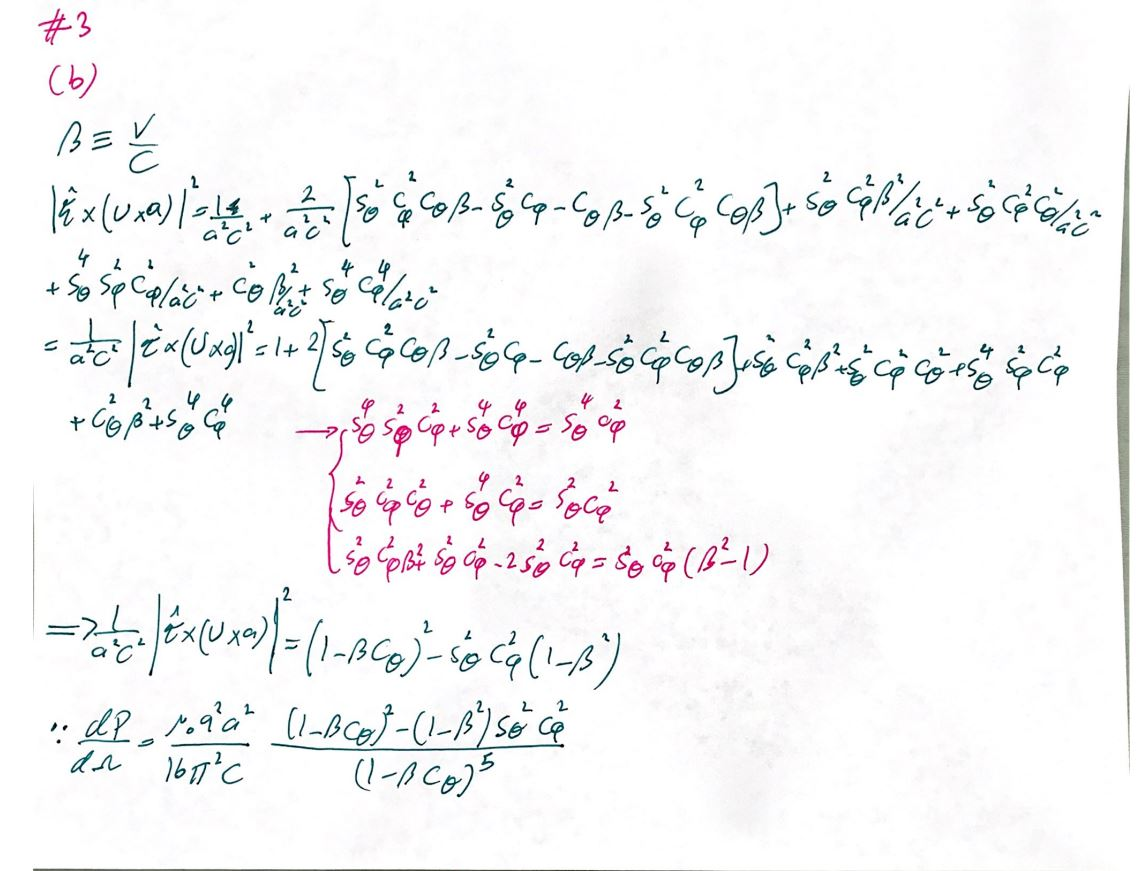
\includegraphics[height=16cm, width=17cm]{3B(A).JPG}
    \end{center}

    \pagebreak

    \begin{center}
      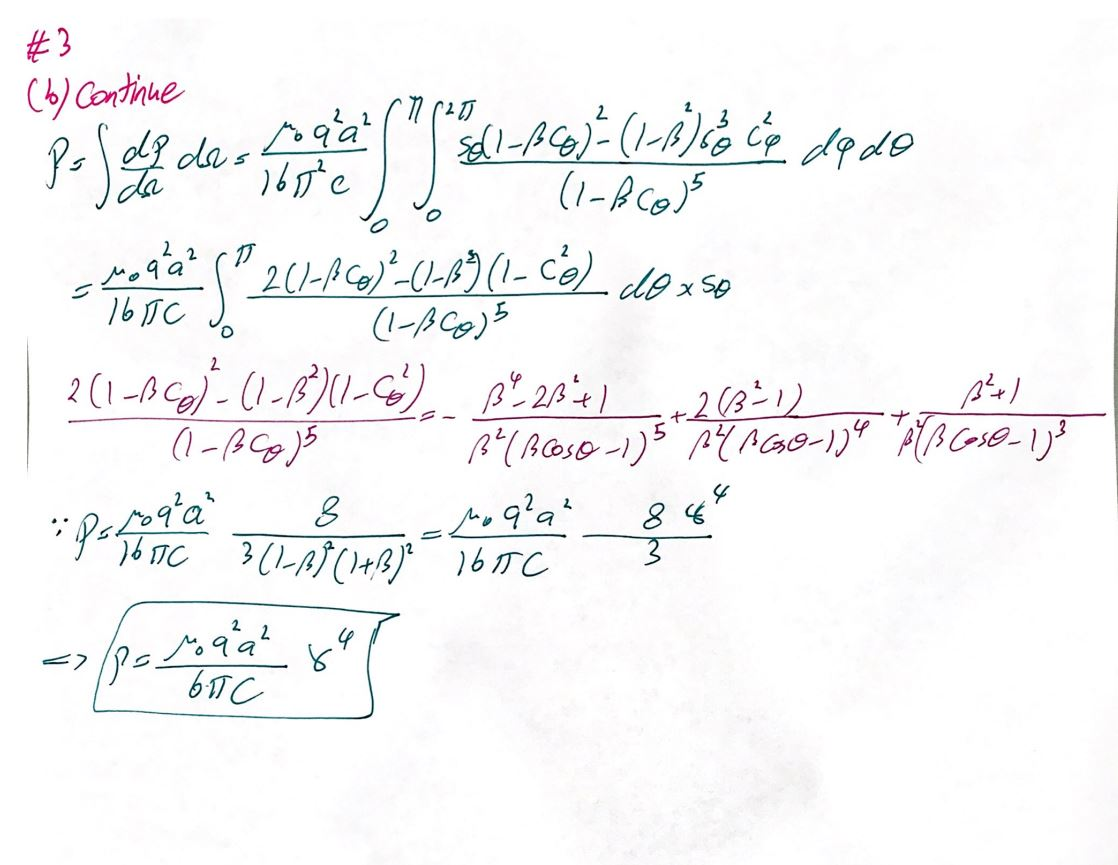
\includegraphics[height=16cm, width=17cm]{3B(B).JPG}
    \end{center}
    
    \pagebreak

    \item \textbf{Problem 4 [25 points]}
    When a linear dielectric sphere of relative permittivity $\epsilon_r$ is placed in a uniform static electric 
    field $E_0$, the field inside of the sphere is uniform and is equal to
    $$
      E_{in}=\dfrac{3}{\epsilon_r+2} E_0
    $$
    according to Griffiths equation $4.49$. From this model, we can develop the theory of Rayleigh scattering.
    Assume the sphere has a radius $R$.
    \begin{enumerate}
      \item Write down an expression for the polarization field $P$ within the sphere, in terms of 
      $\epsilon_r$ and $E_{in}$.

      \item Determine the “polarizability” of the sphere, $\alpha$, defined by the relation $p=\alpha E_0$ 
      where $p$ is the total dipole moment of the sphere. Hint: $P$ is the dipole moment per volume.

      \item Suppose the external field is a plane wave of the form $E_0(r,t)=E_0 cos(kx-\omega t) \hat{z}$ and the
      sphere is situated at the origin. In the Rayleigh approximation, we assume $\lambda >> R$ so that the
      above uniform-field result is reasonable. Determine the electric dipole radiation fields $E_{dip}$ and
      $B_{dip}$ far from the sphere in terms of $\alpha$, $\omega$ and $E_0$. Use the usual spherical coordinates 
      $r, \theta, \phi$ and $\hat{r}, \hat{\theta}, \hat{\phi}$. 
      \emph{Hint: save time by making use of equations developed in Griffiths.}

      \item Determine the power radiated into a distant detector with a tiny solid angle $\Delta \Omega ≪ \pi$. 
      Write it down in terms of $R$, $\epsilon_r$, the angles $\theta$ and $\phi$, and the incident intensity 
      $I_0=\dfrac{1}{2 \mu_0 c}|E_0|^2$. \emph{Hint: save time by making use of equations developed in Griffiths.}
    \end{enumerate}

    \begin{center}
      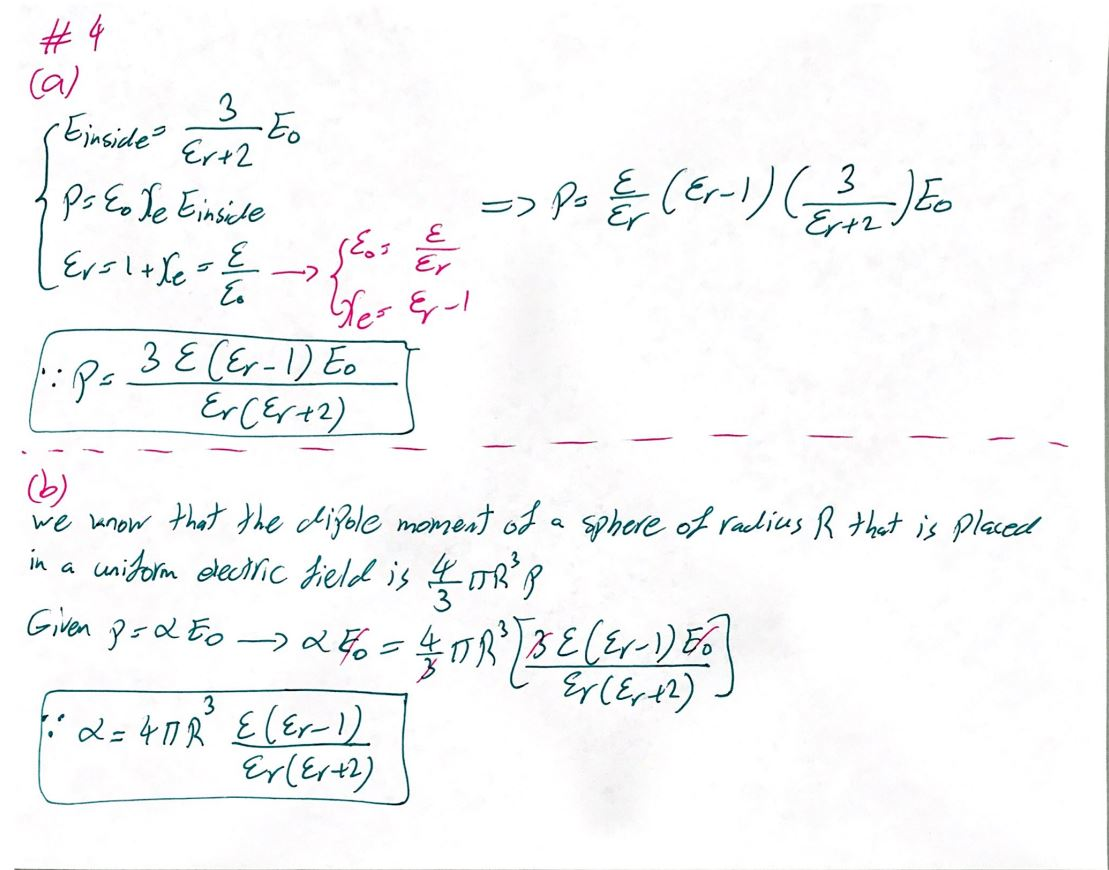
\includegraphics[height=16cm, width=17cm]{4A.JPG}
    \end{center}

    \pagebreak

    \begin{center}
      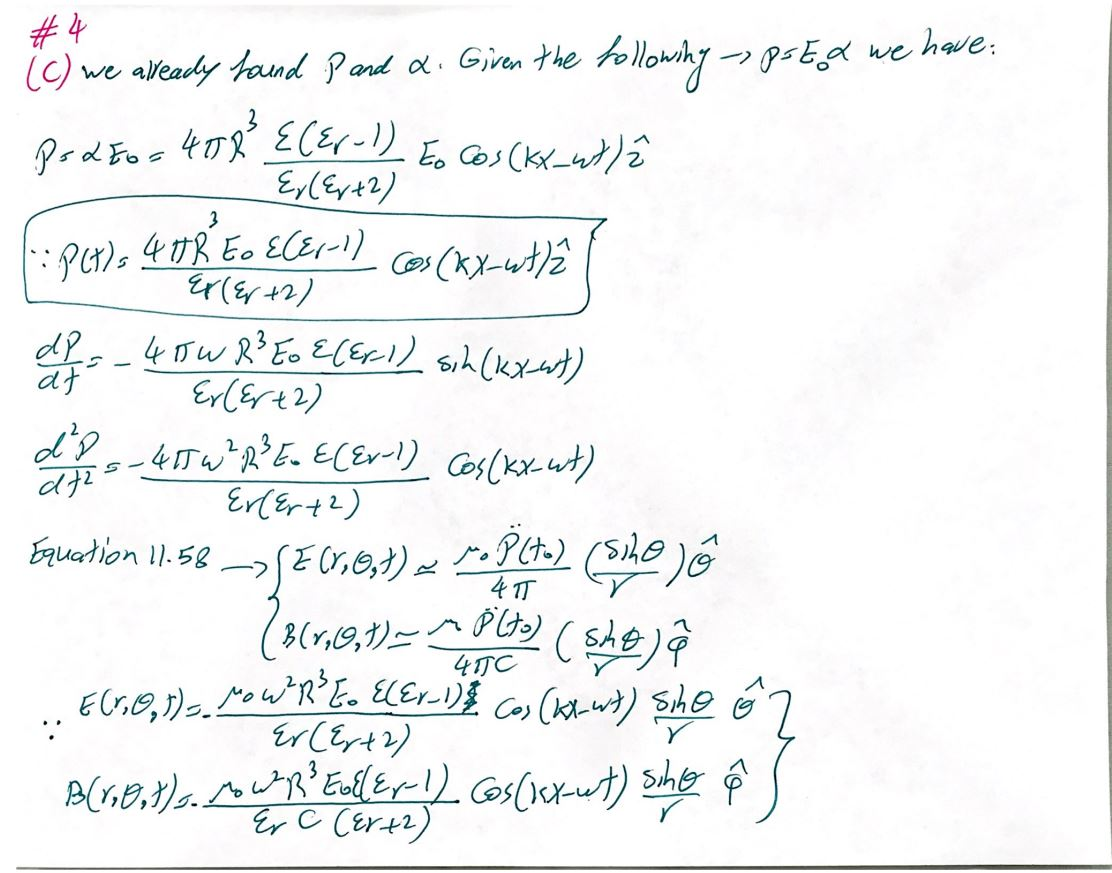
\includegraphics[height=16cm, width=17cm]{4B.JPG}
    \end{center}
    
    \pagebreak

    \begin{center} 
      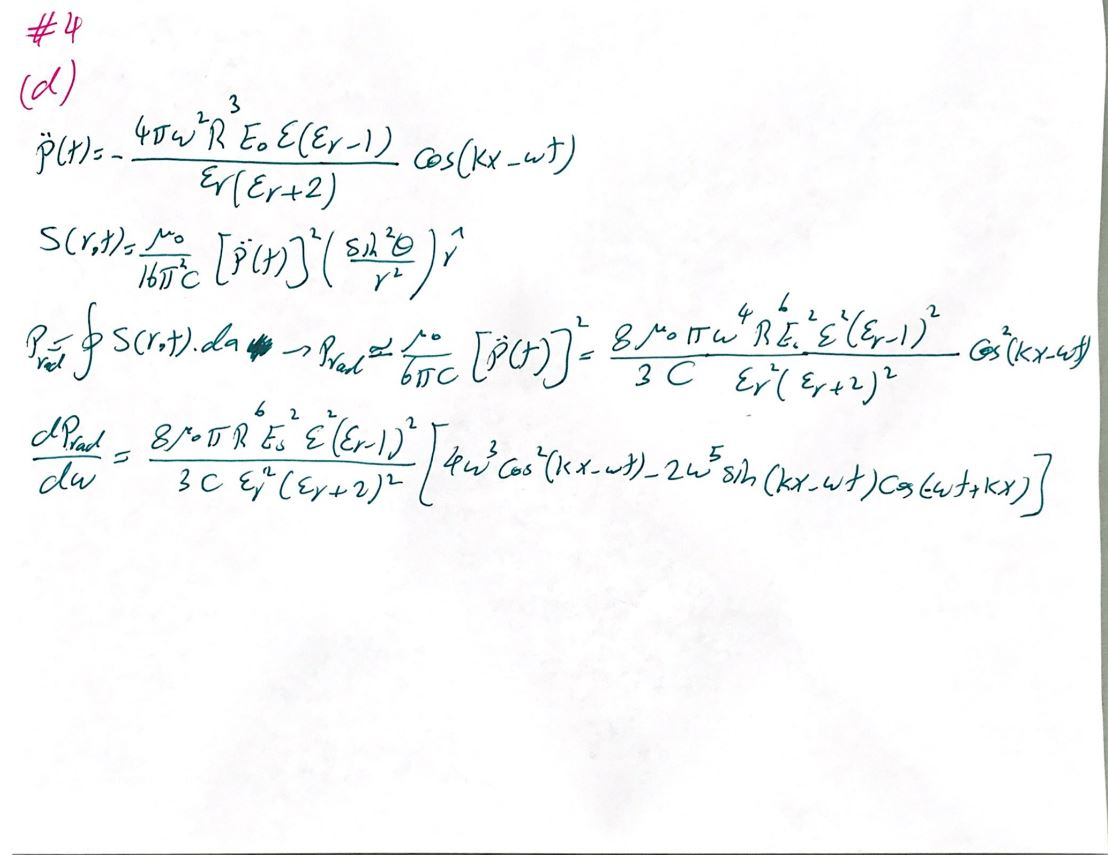
\includegraphics[height=16cm, width=17cm]{4C.JPG}
    \end{center}
    

  \end{enumerate}

\end{document}
